\documentclass{article}

% Language setting
% Replace `english' with e.g. `spanish' to change the document language
\usepackage[english]{babel}

% Set page size and margins
% Replace `letterpaper' with `a4paper' for UK/EU standard size
\usepackage[a4paper,top=2cm,bottom=2cm,left=3cm,right=3cm,marginparwidth=1.75cm]{geometry}

% Useful packages
\usepackage{amsmath}
\usepackage{graphicx}
\usepackage[colorlinks=true, allcolors=blue]{hyperref}

\title{Notes on silhouette-based clustering}
\author{Calvani Tommaso}
\begin{document}
\maketitle

%\begin{abstract}
%Your abstract.
%\end{abstract}

\section*{Questions from first meeting}

\begin{enumerate}
\item Is Silhouette score monotone with respect to the number of clusters? Is it unimodal? Is there any literature regarding Silhouette properties?
\item Can Silhouette score be negative in an optimal clustering?
\item Are silhouette-optimal clusters always separable by a hyperplane?
\end{enumerate}

\section{Mathematical properties of the optimal score with respect to the number of clusters k (Answer to question 1):}

\subsection*{Monotonicity}

There is no literature regarding these properties, it is however immediate to prove that it is not monotone by computing the optimal silhouette score for the 6 points example on \ref{fig:1} and \ref{fig:2}.

\begin{figure}[htbp]
    \centering
    \begin{minipage}{0.45\linewidth}
        \centering
        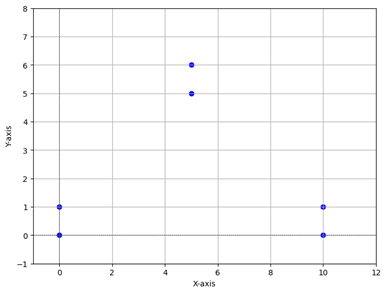
\includegraphics[width=\linewidth]{triangleex.png}
        \label{fig:1}
    \end{minipage}
    \hfill  % Adds some horizontal space between the figures
    \begin{minipage}{0.45\linewidth}
        \centering
        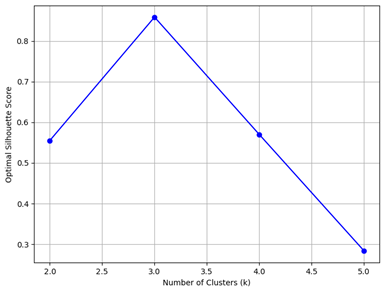
\includegraphics[width=\linewidth]{trianglesil.png}
        \label{fig:2}
    \end{minipage}
\end{figure}

\subsection*{Unimodality}

Intuitively the score is also not unimodal, counterexample is shown in \ref{fig:3} and \ref{fig:4}.

\begin{figure}[htbp]
    \centering
    \begin{minipage}{0.45\linewidth}
        \centering
        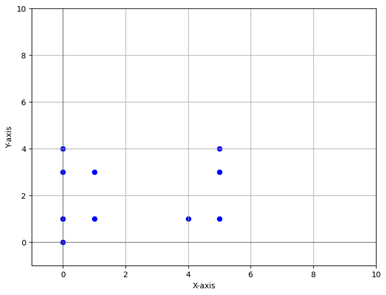
\includegraphics[width=\linewidth]{ex2.png}
        \label{fig:3}
    \end{minipage}
    \hfill  % Adds some horizontal space between the figures
    \begin{minipage}{0.45\linewidth}
        \centering
        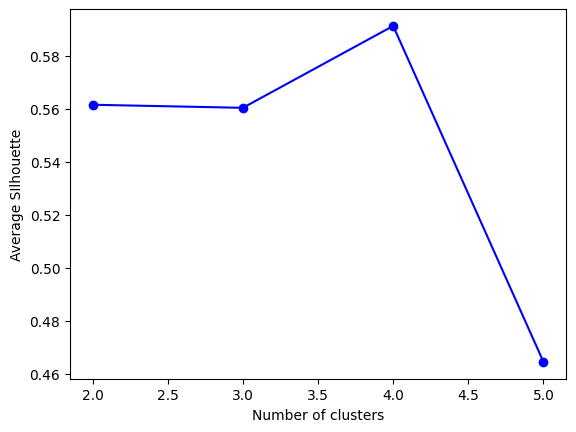
\includegraphics[width=\linewidth]{plot2.png}
        \label{fig:4}
    \end{minipage}
\end{figure}


\section*{Other approaches to silhouette-based clustering in literature:}

Most of the approaches found in literature start from an initial clustering (that could be the result of another algorithm such as k-means) and try to refine this result locally searching for an improvement in the silhouette score. Issues with the complexity of computing this score at each attempt are tackled by using simplified versions of the score (MEDSIL, simplified silhouette) or by working on a subset of the dataset.

\subsection{\textbf{OSil/FOSil} algorithms (Clustering with the Average Silhouette Width, Fatima Batool, Christian Hennig, 2021)}

Starting from an initial clustering, at each iteration reassigns points that give the highest improvement for the average silhouette score. In the other alternative (FOSil), only reallocates a random sample of the dataset and then assigns the rest of the points in order to maximize their individual silhouette score.
Experimental results show that OSil and FOSil return better results than k-means only on some specific synthetic datasets, while not achieving any improvement in most cases (also on real datasets).

\subsection{\textbf{FSMC} algorithm (Medoid Silhouette clustering with automatic cluster number selection, Lars Lenssen , Erich Schubert, 2024)}

Improvement of the PAMMEDSIL algorithm, where to simplify the computation of the silhouette score only the distance to a cluster’s medoid is used instead of the average distance with all the point.
In the paper it is assumed that individual silhouette scores are always non-negative in order to furtherly simplify the silhouette score formula.
The core of the algorithm is still iteratively swapping medoids and normal points searching for an improvement in the average silhouette score.
In particular, in order to reduce the computational costs, the first swap returning an improvement is chosen (“First descent”) instead of the one achieving the largest improvement (“Steepest descent”).
Moreover, the algorihtm start from a maximum number of clusters (kmax) and after each iteration removes the medoid with the lowest contribution to the average silhouette score, resulting in an automatic selection of the number of clusters.
Results show that the algorithm achieves results comparable to PAMSIL with a lower runtime.


\subsection{\textbf{REMOS1 / REMOS2} algorithms (Comparison of silhouette-based reallocation methods for vegetation classification, Attila Lengyel, David W. Roberts, Zoltán Botta-Dukát, 2020)}

The paper compares the existing OPTSIL approach (Roberts, 2015) which searches for the allocations that most increase the average silhouette score of an initial clustering with a new approach that aims to maximize the individual silhouette scores. In particular, at each iteration REMOS1 reallocates to the second closest cluster a fixed number of points with the lowest individual silhouette score, while REMOS2 reallocates all the points with a negative individual score.
The idea is that a negative individual silhouette score implies a misclassification of the point.
The two algorithms are compared on real datasets containing vegetation samples and then evaluated with respect to the average silhouette score achieved and the misclassification rate.
OPTSIL achieved a generally higher average silhouette score compared to REMOS1 and REMOS2, however these two algorithms returned a misclassification rate mostly equal to zero which OPTSIL couldn’t achieve. 

\section*{Observations and questions}

\begin{itemize}
\item In every approach I could see, results never achieve a significant improvement compared to k-means. In general, k-means’ results seem to be a good approximation of the optimal silhouette score (however there are no guarantees about this).
\item \textbf{Question}: when does the silhouette function behaves differently from k-means cost function?
\item As shown in the vegetation classification paper, in some contexts optimizing the average silhouette score doesn’t seem to return the most desireable result, while maximizing the individual scores could be better even if achieving a lower average score.
\item \textbf{Question}: can the optimal average silhouette score be negative? Can the individual scores be negative in an optimal clustering? Does a negative individual score necessarily imply a misclassification? 
\end{itemize}

\section*{Definitions}

\subsection*{Individual Silhouette Score for Point \( i \):}

The silhouette score \( s_i \) for an individual point \( i \) is defined as:
\[
s_i = \frac{b_i - a_i}{\max\{a_i, b_i\}}
\]
where:
\[
a_i = \frac{1}{|C_i| - 1} \sum_{\substack{j \in C_i \\ j \neq i}} d(j, i)
\]
and
\[
b_i = \min_{\substack{C_j \neq C_i}} d(i, C_j)
\]

\subsection*{Average Silhouette Score for the Dataset \( D \):}

The average silhouette score \( S \) for the entire dataset \( D \) is defined as:
\[
S = \frac{1}{n} \sum_{i \in D} s_i
\]

\end{document}